% Chapter Template

\chapter{Product Design} % Main chapter title

\label{Chapter2} % Change X to a consecutive number; for referencing this chapter elsewhere, use \ref{ChapterX}

\section{App Design}
App design combines User interface (UI) and User Experience (UX), while UI concerns about how the app pages look like and feel, such as the fonts, colours and arrangements of icons, UX focuses on the functionality and usability. The best app design process comprises research, ideation, problem identification, design, feedback and problem evaluation. \textbf{(need explanation)} Currently, we only focus on the mobile app design or specifically IOS design based on Apple Platform and Android Design. 

\subsection{UX Design}
UX Design is the process of deciding how someone will use an app and creating a viable product. It’s during the UX process that mobile app design ideas are generated and validated, with an aim to make sure that all your choices are going to work so that our app works. 
\\The quality of user experience is the crucial factor measuring the quality of the design and usually it's the key distinguishing a successful app design from a bad one. Customers are becoming more and more picky about which app to use and so quick to abandon the app which they don not enjoy, so it's essential to invest time and effort in creating a great user experience.
\subsubsection{Minimum Viable Product (MVP)}
A minimum viable product, or MVP, is a product with enough features to attract early-adopter customers and validate a product idea early in the development cycle. To decide which features belong the MVP design, we use MoSCoW method to represent all the features we want to include in our design, while M (Must Have) o S (Should Have) C (Could Have) o W (Won’t Have). 
\\We also take Impact Effort matrix and AARRR framework evaluation method into consideration, where Impact Effort matrix is shown in figure[]. AARRR stands for Acquisition, Activation, Retention, Referral, Revenue. \textbf{need to explain}

\begin{table}[ht]
\centering
\begin{tabular}{ |c|c| } 
 \hline
\textbf{MUST HAVE FEATURES FOR MVP} & \textbf{SHOULD/ COULD HAVE FEATURES}\\ 
 \hline
 Sign-up and sign-in with email & Sign-in with third party accounts \\ 
 \hline
 Upload Audio & Real-time generation \\ 
 \hline
 Chord output & Chord regeneration \\ 
 \hline
 Chord layout &  Export to PDF \\ 
 \hline
 Share posts & Message channel \\ 
 \hline
 Recommendation Engine &  \\ 
 \hline
 Help and support &  \\ 
 \hline
 File storage& File backup \\ 
 \hline
 \end{tabular}
 \caption{MoSCoW Table}
 \centering
 \end{table}
 
 \subsubsection{User Flow and Funtionality}
User flows are flowcharts that illustrate the movement or journey of a user through your app. User flow diagrams are indispensable in mastering user experience. They allow you to understand how users interact with your app or website, the steps they take to complete a task or achieve a goal on your website. This will help you create a superior user experience for the user and meet their needs more efficiently.  
\\There are two user flow diagrams representing two of the most important journey, one is sign-in flow figure[---] and the other one is main function page flow figure[---]. We use rounded rectangle to represent the termination, diamond to represent the decision, rectangle to represent the process and arrow to represent the flow direction.

\begin{figure}
\centering
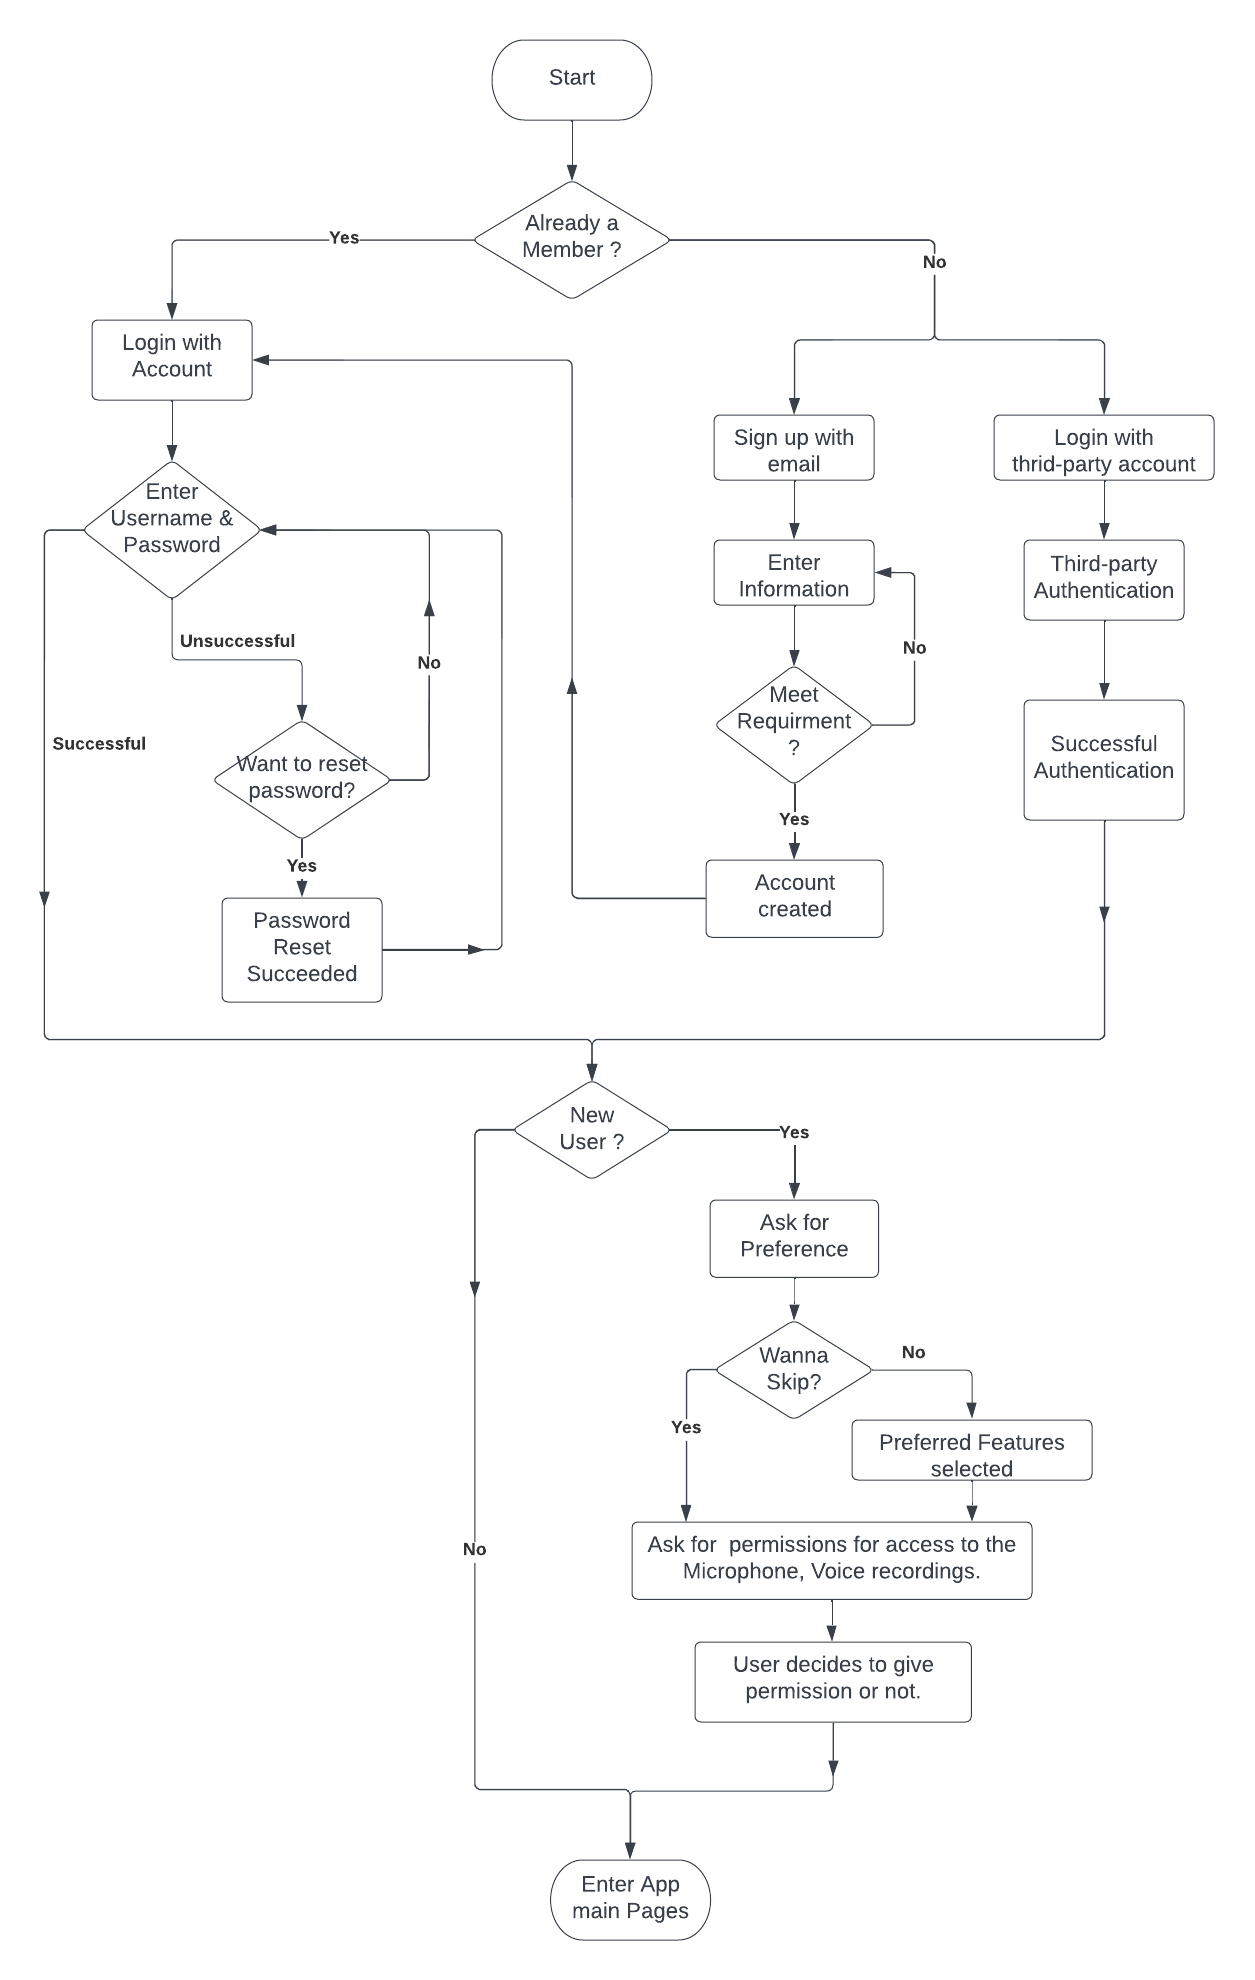
\includegraphics[scale = 0.25]{Flow diagram1.png}
\caption{User Flow Diagram for Login}
\centering
\end{figure}

\subsubsection*{Main Functionality}

\begin{itemize}

\item \textbf{Sign-up and Sign-in with Email}
\\From the start, our user can sig-up with their email and then login in with our app accounts. The reason why we want our user to create an account is that we can profile our users more easily.

\item \textbf{Sign-in with with third-party Accounts}
\\ The purpose is to reduce the barriers for our users to enter our app. OAuth (Open Authorisation) is an open standard for access delegation, commonly used as a way for internet users to grant websites or applications access to their information on other websites but without giving them the passwords.This mechanism is used by companies such as Amazon, Google, Facebook, Microsoft, and Twitter to permit the users to share information about their accounts with third-party applications or websites.

\item \textbf{Ask for song tag preference}
\\After our user sign-in, a question with selective answers will show on the main page, the answers will be stored and feed to our recommendation engine, \textbf{Link to recommendation engine section}.

\item \textbf{Store and backup files on Cloud}
\\The purpose is to enable better synchronisation between devices and accessibility to the files. 
\\We will include CloudKit in our IOS design to allow users to store their saved files in iCloud, (merit: grate integration, recordings can also be stored)
\\

\item \textbf{Recording input}
\\

\item \textbf{Chord generation and regeneration}
Unlike Chordify, which generates the same chords each time for the same audio source, we provides the option for users to regenerate the chords and we aim to provides sightly different chords when regeneration button is pressed.

\item \textbf{Share works in the community page}


\end{itemize}

\begin{figure}
\centering
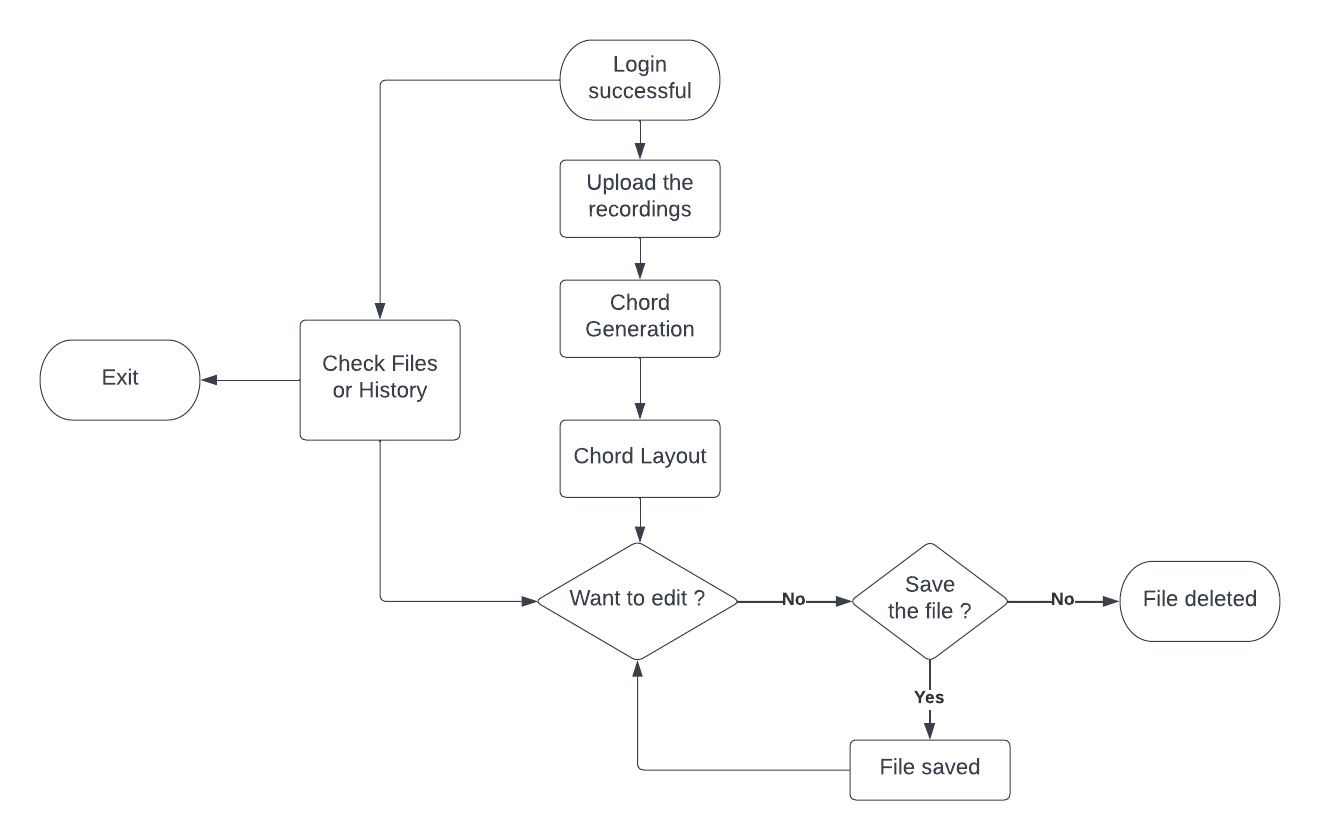
\includegraphics[scale = 0.25]{MFpage.png}
\caption{User Flow Diagram for main function page, figure need to be improved here}
\end{figure}



\subsection{UI Design}
After having the map of user flow, we started to design the prototype using Figma.

\begin{figure}[ht]
     \centering
     \hspace{16mm}
     \begin{subfigure}[b]{0.2\textwidth}
         \centering
         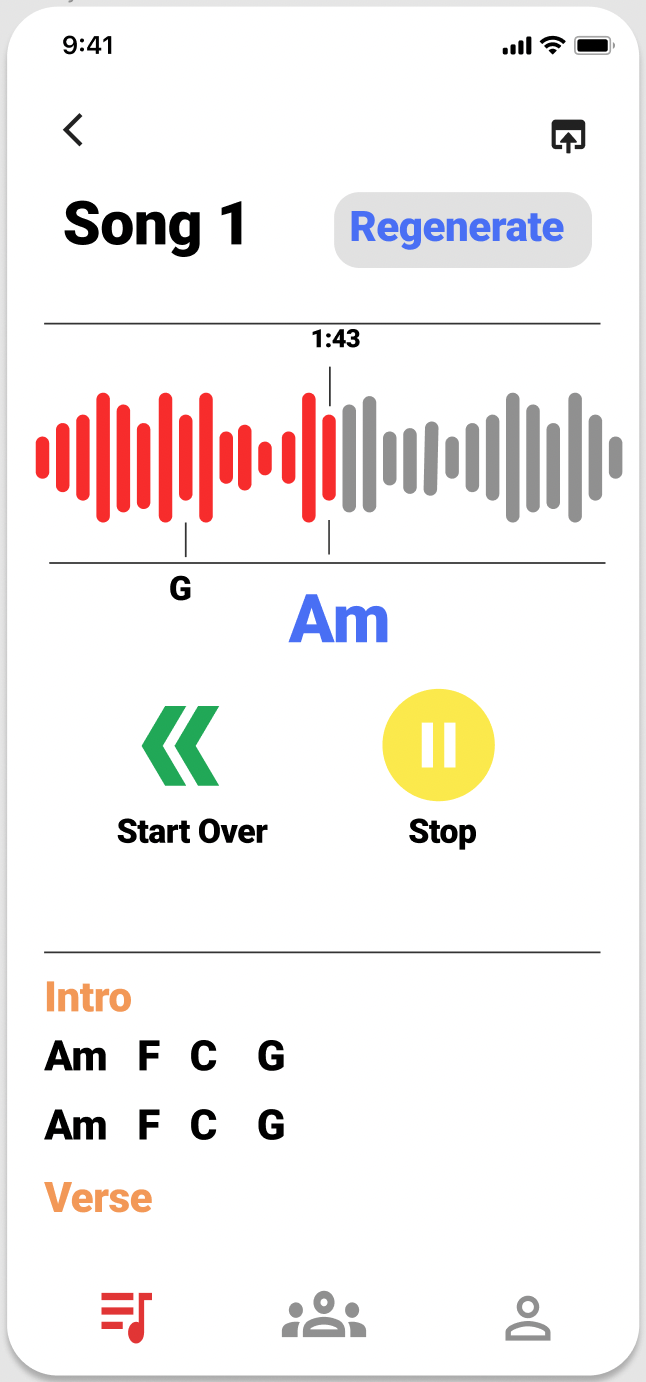
\includegraphics[width=\textwidth]{grappp}
         \caption{Log-in page}
         \label{Log-in page}
     \end{subfigure}
     \hfill
     \begin{subfigure}[b]{0.2\textwidth}
         \centering
         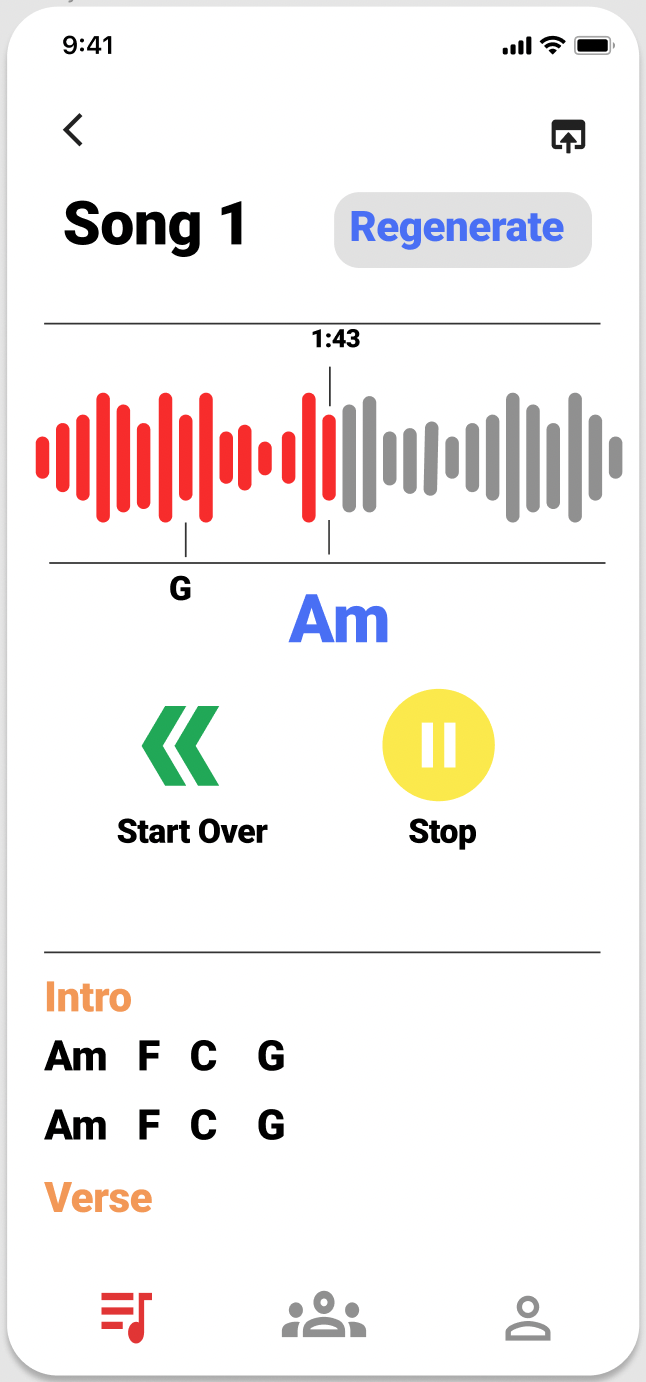
\includegraphics[width=\textwidth]{grappp}
         \caption{Main function page}
         \label{Main function page}
     \end{subfigure}
     \hfill
     \begin{subfigure}[b]{0.2\textwidth}
         \centering
         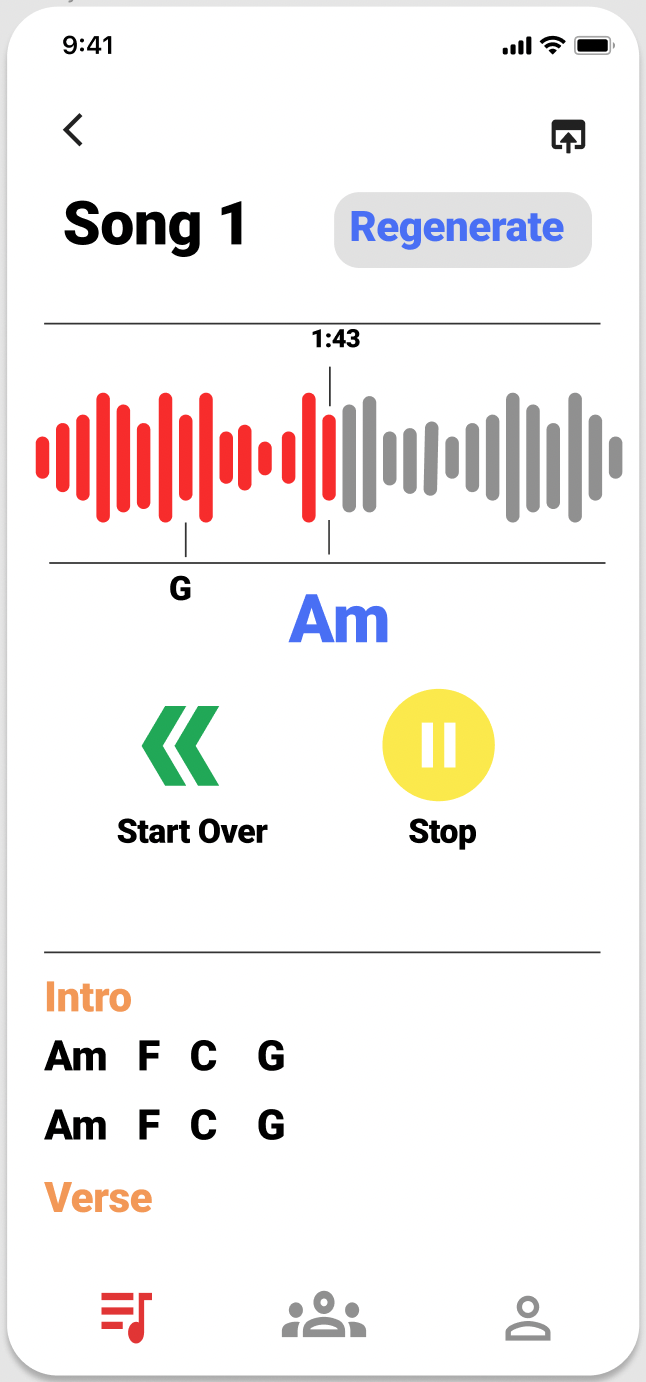
\includegraphics[width=\textwidth]{grappp}
         \caption{Community page}
         \label{Community page}
     \end{subfigure}
     \hspace{16mm}
        \caption{UI design for our app}
        \label{fig:three graphs}
\end{figure}

\subsection{Testing}

\subsection{Programming and Data architecture}
End point design
\\talk about some security here to link with data security section
